\documentclass{article}

\usepackage{subfigure}
\usepackage{graphicx}

\date{}
\pdfpagewidth=8.5truein
\pdfpageheight=11truein

\addtolength{\oddsidemargin}{-.875in}
\addtolength{\evensidemargin}{-.875in}
\addtolength{\textwidth}{1.75in}

\addtolength{\topmargin}{-.875in}
\addtolength{\textheight}{1.75in}


\begin{document}

\title{Vision Component Documentation \\ Evan Krause \\ 06/2014}
\maketitle

\section{Overview}
This document is intended to make usage and continued development of
the ADE Vision Component as painless as possible. I will start by describing
how to build things on a new machine, and how to configure and run
various setups. For those of you that wish, or need, to continue the development
of the vision component and add functionality, I'll then give a high-level
overview of the code structure, followed by specific directions on how to
integrate new features (e.g., detectors, trackers, etc.).

Also, you'll have the best chance of getting everything running on Ubuntu.
Things have only been tested on Ubuntu (12.04 in particular, but other
versions should also work), and vision also makes heavy use of 
third-party libraries that have been targeted at Ubuntu.

\section{Using the Vision Component}
The first thing to do is checkout the vision code. This requires getting code
from two separate git repositories, one for the main ADE codebase, and one for
the ADE-Vision codebase. Information for getting the code, the dependencies,
compiling, running, and troubleshooting is documented on the HRI Lab wiki
(www.hrilab.tufts.edu/wiki), so I won't duplicate that information here.

\subsection{Configuring Vision}
Now that you have vision running on your machine, I'll discuss various
ways to configure vision without making any code changes. Most of these options
will be set via the command line while starting the vision component
(i.e., by using -Dargs="" when starting the component). All of the available
options can be seen by running vision with the help flag
(i.e., ./ant run-visioncomponent -Dargs="-help"), but I will mention a few key
options below.

\subsubsection{Sensor Options}
Vision supports a wide variety of sensor inputs (e.g., single camera, stereo camera,
Kinect, video recording, static image, etc.). By default, Vision attempts to find
and use a single camera. Use the help flag to see all the "-cammode" options.
I've attempted to filter out available vision capabilities automatically based
on the sensor selection, so using a Kinect, for example, will provide more capabilities
because there is depth information (RGB-D).

\subsubsection{Vision Coordinate System}
Certain Vision capabilities need to have information about where the sensor is located
in the real world (i.e., 2 meters off the ground, looking down at 45 degrees). Table
plane detection, for example, needs this information to distinguish between wall planes,
floor planes, and likely table planes. This information can be set using the "-height"
and "-rotX" arguments. When the sensor is mounted on a robot, however, simply 
setting these values as static might not suffice. If the sensor will be moving 
relative to other parts of the robot, this information needs to be updated dynamically.
This is often the case when the robot needs to manipulate an object that has been
detected and tracked by Vision, or when the vision sensor will be moving (e.g., mounted
on a moving head). Both the MDS and PR2 components contain information about the
coordinate frames for each joint and sensor, and using the "-mds" or "-pr2" flag
will dynamically retrieve the sensor coordinate frame information from
the MDS or PR2 component, respectively.

\subsubsection{Configuration Files}
\label{sec:config_files}
There are a handful of configuration files that are loaded by default during start-up.
They determines all the vision capabilities available to the system, information
about how each capability should be instantiated (e.g., what RGB ranges are red),
and where appropriate, the predicates that are used to advertised those capabilities
to the rest of the system (see Section~\ref{sec:predicates} for more info on predicates in Vision).

The command line options allow different config files to be used, but the default
files live in the $<$ADE-Vision-Home$>$/native/data/ directory. Each of the default files
contains documentation at the top about how to use each file. These files specify
the available Detectors (--detectConfig), Trackers (--trackConfig), ImageProcessors
(--imgProcConfig), SaliencyProcessors (--saliencyConfig), and ValidationProcessors
(--validationConfig). For more complicated vision searches that involve
lots of separate vision capabilities (e.g., search for a medkit), pre-built searches
can be specified in the searchTypes config (--searchConfig).

\subsubsection{Logging}
Another important configuration step is the logging configuration. Vision uses two different
logging systems; log4j for the Java code, and log4cxx for the native code. The Java logging
is done the same way as the rest of ADE, so I'll refer you to the wiki for more information
about log4j, and how to set that up. The native logging config file is set using the
--logcxxConfig argument, and uses the $<$ADE-Vision-Home$>$/native/data/logging/log4cxx.txt
file by default.

Please, please, please, learn what the various logging level mean and learn how to use
logging correctly. A lot of time has been put into integrating proper logging mechanisms,
and it will save you so much time and effort if you continue to use them correctly. System
prints and std out are the devil in large systems!

\subsection{A Word on Predicates - type(X,word) $\wedge$ type(Y,predicate) $\wedge$ relation(X,Y,on)}
\label{sec:predicates}
There have been a lot of predicate related issues when trying to integrate ADE
components, largely due to disparate use of predicates in the various components,
so I thought it would be useful to briefly describe how predicates are currently
used in Vision. First, as mentioned in Section~\ref{sec:config_files}, all the predicates
used are defined in the various config files. Additionally, Vision makes certain
assumptions about the form of predicates, namely that the descriptor is always the
last argument (e.g., red in color(X,red), on in spatial relation(X,Y,on)), and
the functor name is a higher-level "category" (e.g., color in color(X,red), spatial relation
in spatial relation(X,Y,on)). 

It's also worth noting that when parsed from a string (as is the case when parsing
the config files),"?X:" represents a Variable, "X:" a Constant, and "X" a symbol.
This is important in the Vision Component because visual searches are only
instantiated in an attempt to find objects to satisfy free variables
(e.g., color(?X:,red)). So, when calling Vision from another ADE component, 
be sure that the free variables are actually com.Variables, and not just com.Symbols
with a variable name like "X".

\subsection{The Vision GUI}
The Vision GUI is the easiest way to familiarize yourself with the functionality of
the component. This is not an ADE GUI, and is not started with the "-g" flag. The main
GUI and Frames Per Second (FPS) GUI pop up by default, but can be hidden with
the "-hideControls" flag. There are four main tabs, and I will briefly describe each
one here.

Tab 1: This is to build new vision searches. You can either create a new Empty search and
fill it in by typing in predicates via the Add Constraints text box, or you can 
instantiate pre-built searches defined in the searchTypes.xml config.

Tab 2: This tab can also be used to instantiate searches, but only SimpleSearches
can be built here. More complex hierarchical searches need to be build on Tab 1. You
can also start various image processors here without needing to instantiate full
visual searches and is useful for debugging purposes.

Tab 3: This is where you can load, save, and define blob colors for the blob detector.

Tab 4: This is the camera calibration tab that can be used to calibrate both
intrinsic and extrinsic camera parameters. This is especially useful if you have
a stereo camera setup and need to calibrate things to get depth information.

Tab 5: Here, you can take snapshots and record video (RGB and/or RGB-D) which can
be used as sensor input instead of live feeds which is really helpful for debugging.

\subsection{Calling the VisionComponent API}
The VisionComponent API is well documented in the code, so generating the Java Docs
or just opening up the code is your best bet. One key thing to understand
is the difference between {\em types} and {\em tokens}. Types are generic categories, like
"mugs" or even "white mug with a handle on the side". Tokens, however, are specific
instances of the type. So, when Vision is tasked with finding objects of type mug
(i.e., type(?X:,mug)), a token representing a particular instance of a mug
will be created (i.e., a MemoryObject) when a mug has been detected.

\section{Adding New Vision Functionality}
For those of you brave enough to continue developing Vision, this section
is intended you give you a high-level overview of the code, the program flow,
and hopefully outline the steps necessary to add new {\em ImageProcessors},
{\em Detectors}, {\em Trackers}, and {\em SearchManagers}.

\subsection{The Build System}
Vision's build system is spread across three different locations and uses
Ant for building Java, and CMake for building C/C++ and SWIG code. The entry
point is the same as the main ADE Ant build system, where all the other ADE components 
are built and run ($<$ADE-HOME$<$>/build.xml). From there, the vision specific
Ant target is called ($<$ADE-Vision-HOME$>$/java/build.xml), which builds the Java side
of the vision repo. And finally, from there, CMake is called to build the C/C++ and
SWIG code (main CMake entry point is located at $<$ADE-Vision-HOME$>$/native/CMakeLists.txt).

\subsection{High-Level Architecture and Program Flow}
The high-level overview can be seen in Figure~\ref{fig:vis_arch}. The most important
classes are the four factory classes; {\em AvailableSearchManagers},
{\em AvailableImageProcessors}, {\em AvailableDetectors}, and {\em AvailableTrackers}.
AvailableSearchManagers is responsible for constructing and handing out
{\em SearchManager} instances, where a SearchManager is a single visual search.
To construct a new SearchManager, the AvailableSearchManagers tries to 
satisfy all the free variables contained in the passed in predicates by
consulting the other factories (or by checking if an existing SearchManager
is appropriate). The other factory classes work in a similar fashion by
creating and handing out ImageProcessors, Detectors, or Trackers if they
meet the particular request of AvailableSearchManagers. It's worth noting that
there are actually three separately instantiated AvailableImageProcessors classes,
one to manage and create SaliencyProcessors, one for ValidationProcessors, and one
for all other ImageProcessors. All the factories are instantiated in the 
Vision.java class and the options available in each factory are populated
by the various config files mentioned in Section~\ref{sec:config_files}.

Once the AvailableSearchManagers factory has successfully assembled
the necessary VisionProcessors for a requested visual search, the instantiated SearchManager can
be handed out. The specifics of a SearchManager depend on the kind
of visual search required. Currently there are three kinds of SearchManagers
available to the system; {\em SimpleSearchManager}, {\em RelationSearchManager}, 
and {\em ComposedSearchManager}. The SimpleSearchManager is composed of a
Detector, Tracker, and zero or more ImageProcessors. This is the most basic
kind of search and is currently used the most often. A RelationSearchManager
is composed of two SimpleSearchManagers, a Detector, and a Tracker,
and is used for hierarchical searches such as "white box with a red
cross on it." Here, the "white box" and "red cross" are both
SimpleSearchManagers and the results of those two searches are consumed
by the Detector to search for the "on" relationship. The ComposedSearchManager
is not currently used but is intended for even more complex searches.

If you're wanting to add a new search capability into the Vision Component,
and it doesn't fit nicely into one of these existing SearchManager types,
it's likely that you'll need to add a new class by extending the SearchManager
base class with specialized functionality.

\begin{figure}[t]
  \centering
  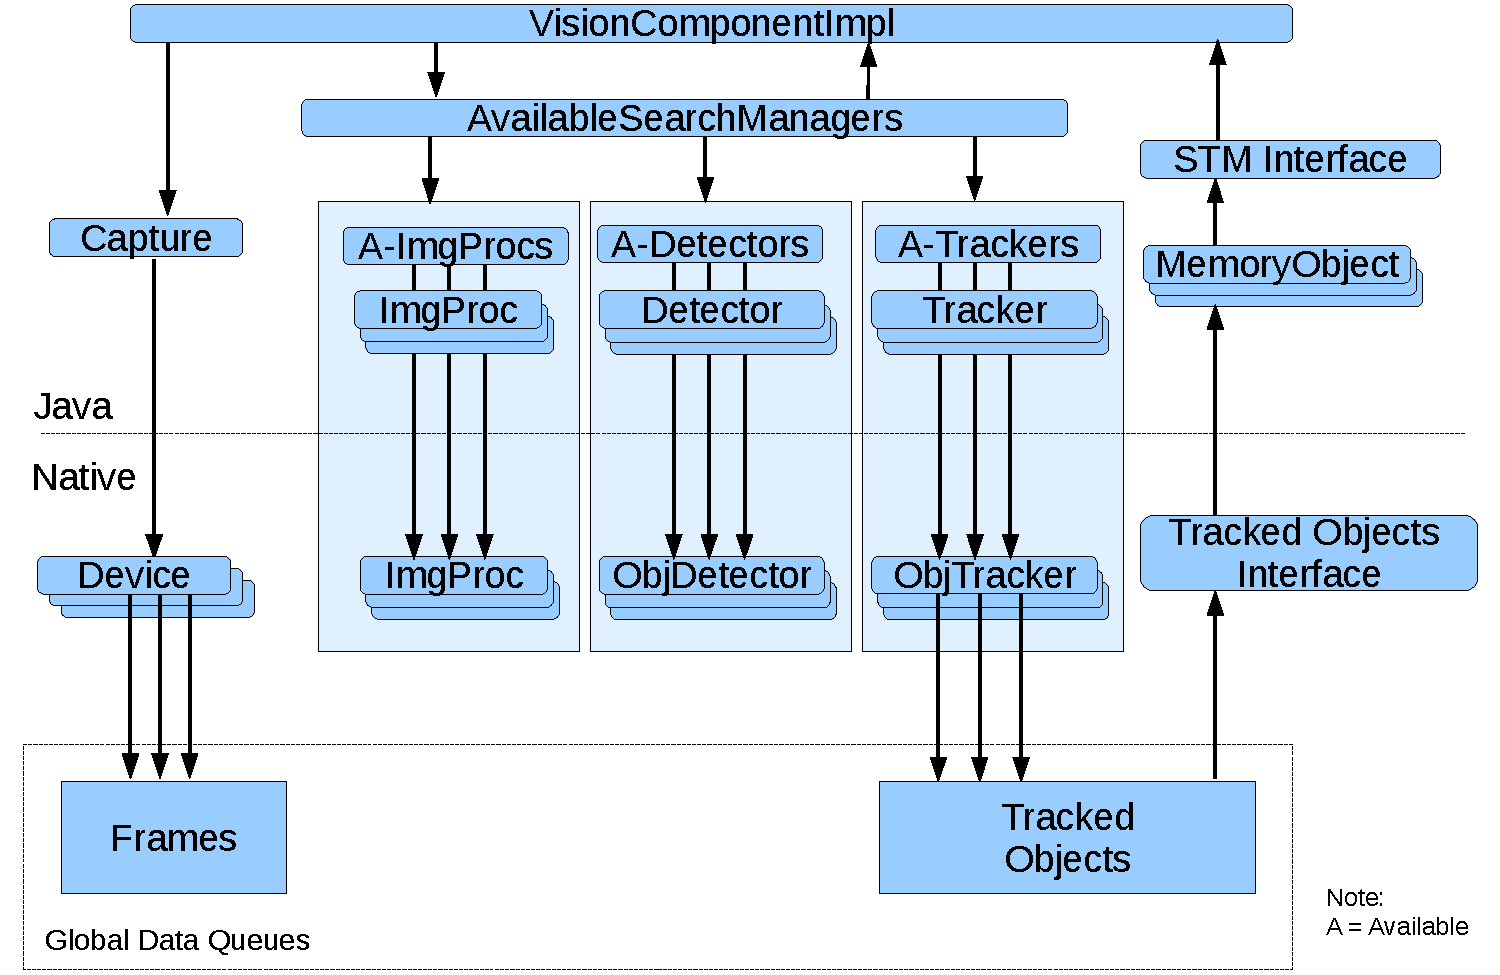
\includegraphics[width=7.0in]{vision_arch.pdf}
  \caption{High level vision system architecture.}
  \label{fig:vis_arch}
\end{figure}

\subsection{Core Class Hierarchy}
So far, I've only discussed how a visual search is constructed, the various
classes involved, and the high-level program flow. The core of the actual
vision processing (i.e., pixel and point cloud twiddling) takes place within
the {\em ImageProcessor}, {\em Detector}, and {\em Tracker} classes. The
SearchManagers discussed above contain various combinations of these
three Java classes which themselves contain pointers to their C++ counterparts.
All of the image and point cloud processing takes place on the C++ side,
so we'll turn our focus there. All processing classes (except for the Capture
classes) are derived from the same VisionProcess class, and the full inheritance
diagram can be seen in Figure~\ref{fig:vis_hierarchy}. This common ancestor allows
for easy communication between the various processors, and enables a common
registration and notification framework.

\begin{figure}[h]
  \centering
  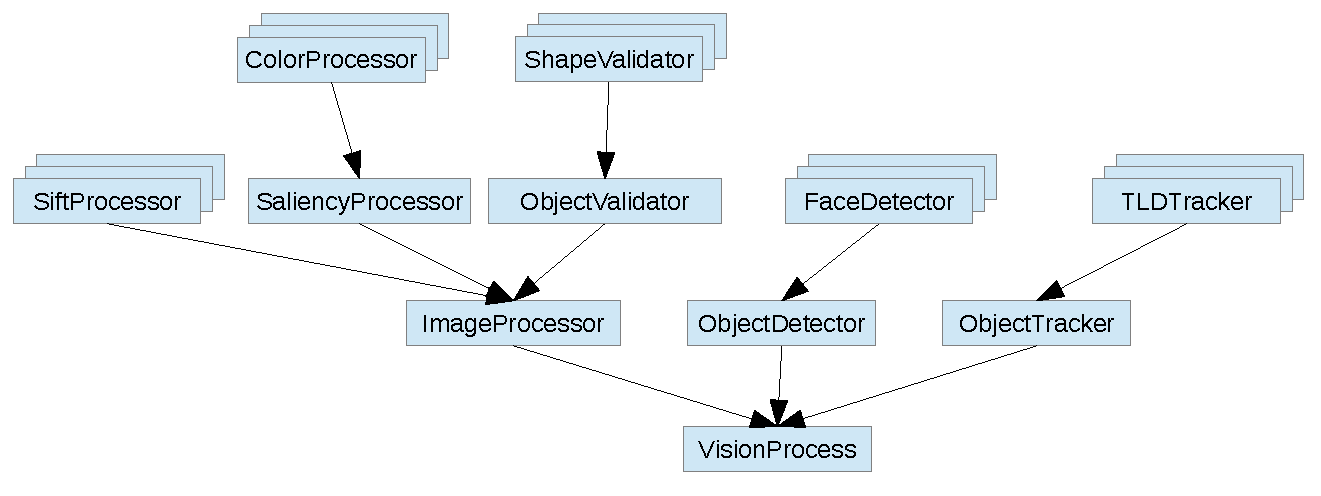
\includegraphics[width=4.5in]{vision_main_hierarchy.pdf}
  \caption{Main vision processor class hierarchy.}
  \label{fig:vis_hierarchy}
\end{figure}

All processors are instantiated from the Java side (as part of a SearchManager),
and registration for notifications between processors also takes place on the Java side
in the SearchManagers. Registration is intended to be fairly automatic, so no additional
work should be needed when adding new ImageProcessor, ObjectDetector, or ObjectTracker
capabilities as long as the config files are set up properly.

Lastly, it's important to understand that the work of each processor is performed
inside its own dedicated thread. Each thread is created and controlled on the Java
side, inside the VisionProcess.java class. The Java ImageProcessor, Detector, and
Tracker classes inherit from the VisionProcess class, resulting in a inheritance
structure that mirrors the C++ structure in Figure~\ref{fig:vis_hierarchy}.

{\em To add a new ImageProcessor, Detector, or Tracker, please take a look at the step-by-step
instructions on the Vision Component wiki page in section titled Contributing to ADE-Vision.} 

\end{document}
